\documentclass{article}
\usepackage[icelandic]{babel}
\usepackage[T1]{fontenc}
\usepackage[utf8]{inputenc}


\usepackage{subfig}

\usepackage{todonotes}
\usepackage{color}

%Leitað er af myndum í eftirfarandi möppum
\graphicspath{{./technical/}{./sprettir/}}
\linespread{1.5}
%\setcounter{tocdepth}{2}

\usepackage{graphicx}
\usepackage{wrapfig}
\usepackage{float}
\usepackage{verbatim}
\usepackage[none]{hyphenat}





\begin{document}
\raggedright

\tableofcontents
\newpage

\section{Inngangur}
Skýrsla þessi er um lokaverkefni í Tölvunarfræði við Háskólann í
Reykjavík, 
sem unnið var í samvinnu við DataMarket. Verkefnið snérist um að hanna kerfi til að greina
breytingar á tímalínum, í gagnasafni DataMarket, sem gætu bent til þess að um markverða eða áhugaverða þróun sé að ræða.

Í skýrslunni lýsum við verkefninu ítarlega og hvernig verkáætlun var háttað.
Einnig segjum við frá þeim reikniaðferðum sem skoðaðar voru með tilliti til 	
lausnar verkefnisins og greinum frá niðurstöðum okkar. Þá 
verður farið yfir atriði sem skoða mætti við nánari þróun kerfisins.
Að lokum er yfirlit yfir framvindu verksins.

\newpage
\section{Lýsing verkefnis}
\label{sec:description}
DataMarket er fyrirtæki sem tekur sama töluleg gögn frá opinberum
stofnunum og einkaaðilum, gerir þau aðgengileg á einum stað og birtir þau á
auðskiljanlegan máta. Þann 25. janúar 2011 samanstóð gagnasafn þeirra 
af meira en 13.000 gagnasettum sem innihélt næstum 100 milljón tímalínur og 
fer það ört vaxandi. Hvert gagnasett hjá DataMarket inniheldur tímalínur sem sýna þróun tölulegra
gagna og getur innihaldið allt að nokkur þúsund tímalína. 
Á hverjum degi eru tugir, eða jafnvel hundruð slíkra gagnasetta uppfærð í
kerfinu. Sú þróun sem ein tímalína sýnir getur verið allt frá vel þekktum gildum t.d. verðbólgu, atvinnuleysi eða
hitastigi í Reykjavík, til mjög sérhæfðra eða jafnvel undarlegri hluta eins og 
innflutningsverðmæti leðurvara frá Brasilíu! 
Mikið er fylgst með algengustu tímalínunum og stórvægilegar breytingar 
í þeim rata iðulega í fréttir umsvifalaust. 
En mjög markverð, áhugaverð eða jafnvel varasöm þróun getur líka birst 
í gögnum sem fáir fylgjast með og jafnvel enginn tekur eftir. 

Þar sem óhagkvæmt er að fara handvirkt í gegnum þetta mikið magn af gögnum 
til að finna áhugaverða atburði, var þörf á sjálfvirku kerfi til að 
sinna því hlutverki og fólst verkefni okkar í að útfæra það.
Upprunalega var kerfið hugsað á þann veg að það myndi athuga hvort ný gögn, sem
væri verið að bæta við tímalínur DataMarket, væru áhugaverð eður ei. Hinsvegar
varð ljóst í þróunarferlinu að kerfið okkar gæti gert meira en unnið
eingöngu með nýjustu uppfærslurnar og varð það því yfirgripsmeira en
upprunalega stóð til.
Óskir DataMarket voru að fyrst yrði útbúið einfalt kerfi sem myndi jafnvel 
skila af sér mikið af ómarktækum niðurstöðum (e. false positives). Það var hugsað
sem grunnur sem hægt væri að byggja á. Því næst átti að þróa og greina aðferðir við
að bæta niðurstöðurnar. 


\newpage

\section{Verkskipulag}


\subsection{Aðferðafræði}

Ekki reyndist unnt að skipuleggja verkefnið í heild sinni í upphafi þar sem hluti þess fólst í að rannsaka hentugar aðferðir við að greina gögn.
Því töldum við Scrum aðferðarfræðina henta okkur vel, sérstaklega sá eiginleiki að geta beðið með ákvarðanatöku þar til hún átti við.

\subsubsection{Kröfulisti}
Byrjað var á því að útbúa einfalda frumgerð sem var síðan betrumbætt.
Útfrá því var verkefninu skipt upp í tvo fasa. 
Sá fyrri stóð yfir fyrstu tólf vikurnar og var hugsaður til að búa til frumgerð af kerfinu.
Seinni fasinn stóð yfir síðustu þrjár vikurnar og var hugsaður til áframhaldandi þróunnar á reikniaðgerðum.
Beðið var með að skipuleggja seinni fasann þangað til að athugannir okkar á reikniritum voru farnar að skila niðurstöðum. 
Því vorum við með tvískiptan kröfulista\footnote[1]{Sjá nánar í 
um produckt backlog í framvinduskýrslu á meðfylgjandi geisladisk}.

\subsubsection{Hlutverkaskipting}

Meðlimir hópsins tóku að sér hlutverk eins og gert er í Scrum. Hlutverkin voru eftirfarandi:

\vspace{5 mm}
\begin{tabular}{| l | l |}
\hline
Titill & Nafn \\
\hline \hline
Scrum meistari & Þórður Bjarki Arnarson\\
\hline
Fulltrúi verkkaupa & Hjálmar Gíslason hjá DataMarket\\
\hline
Forritarar & Allir \\
\hline
\end{tabular}
\vspace{5 mm}

Ekki þótti ástæða til að fulltrúi 
DataMarket kæmi að ákvarðanatöku fyrr en í seinni fasa og því var Arnór Barkarson 
valinn fulltrúi hans fyrir fyrri fasa.

\subsubsection{Sprettir}
\label{sec:sprettir}
Alls var tímabilinu skipt niður í níu spretti. Í fyrri fasa voru sex 
tveggja vikna sprettir og í þeim seinni þrír. Í sjötta spretti gerðum við ráð fyrir lokaprófum og var hann því
skipulagður á fjögurra vikna tímabili, 
en tvær af þeim fóru í prófin. Prófatafla lá ekki fyrir við skipulagningu og því 
var þessi háttur hafður á. 

\subsubsection{Athafnir}

Við notuðum eftirfarandi athafnir við skipulagninu og umsýslu verkefnisins.
Þessar athafnir voru: 

\begin{itemize}
\item Daglegir fundir (e. daily Scrum)
\begin{itemize}
\item Stuttur fundur sem haldin var á hverjum vinnudegi. Þar sagði hver hópmeðlimur frá sínum verkefnum, hvað hann var að gera síðasta vinnudag, hvað hann ætlaði að gera þann í dag og hvort e-ð stæði í vegi fyrir því að hann gæti gert það. Samkvæmt hefðum Scrum voru allir hópmeðlimir standandi á fundunum.
\end{itemize}
\item Skipulagsfundir spretta (e. sprint planing)
\begin{itemize}
\item Sögur valdar fyrir viðkomandi sprett. Sérhver saga brotin niður í verkefni og áætlaðir tímar á hvert þeirra. 
\end{itemize}
\item Gagnrýnisfundir spretta (e. sprint retrospective)
\begin{itemize}
\item Fundur sem var haldinn í lok hvers spretts og þar var farið yfir viðkomandi sprett, hvað okkur fannst ganga vel og hvað illa. 
\end{itemize}
\end{itemize}

\subsubsection{Skjölun}

Haldið var utan um alla skjölun s.s. kröfulista, framvindurit (e. burndown) og dagbækur\footnote{Sjá Framvinduskýrslu á meðfylgjandi geisladisk}
 hópmeðlima á Google Docs. 

Notast var við Scrum vegg þar sem sögur og verkefni tengd þeim voru hengd upp til að fá yfirsýn 
yfir framvindu sprettanna. Að hafa skjölun ávallt í augsýn gaf góða raun og hélt mönnum við efnið.

\subsection{Tímaskipulag}
Eitt af því fyrsta sem við gerðum var að ákveða hvenær 
vikunnar unnið yrði að verkefninu.
Viku skipulagið leit svona út:

\vspace{5 mm}
\begin{tabular}{| l | l |}
\hline
  Mánudagar & 12 - 3 \\
  \hline
  Þriðjudagar & 9 - 17 \\
  \hline
  Miðvikudagar & ekkert unnið\\
  \hline
  Fimmtudagar & 12 - 4 \\
  \hline
  Föstudagar & 9 - 12\\
\hline
\end{tabular}
\vspace{5 mm}

Farið var eftir þessu skipulagi fyrstu tólf vikurnar. 
Í prófatíma lá vinna við verkefnið niðri. 
Að loknum prófum voru þrjár vikur sem meðlimir hópsins gátu einbeitt sér alfarið
að verkefninu. Sett var upp áætlun um að vinna í átta tíma á dag, sjö daga
vikunnar. Yfirlit yfir tímaáætlun má sjá á mynd~\ref{fig:timeplan}

Í þessari áætlun eru ekki meðtaldir tímarnir sem fóru í undirbúning verkefnisins, þ.e.
þegar við funduðum með Hjálmari Gíslasyni hjá DataMarket og að settum saman
lýsingu verkefnisins haustið 2010.

\begin{figure}[H]
  \centering
  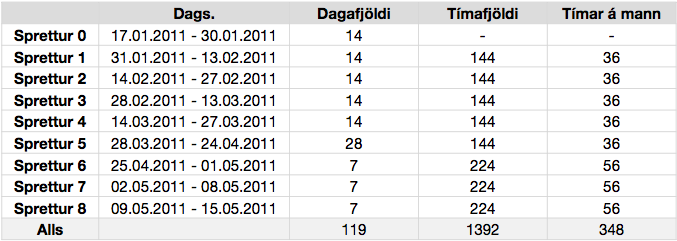
\includegraphics[width=1\textwidth]{sprettir_timar.png} 
  \caption{Tímaáætlun} 
  \label{fig:timeplan}
\end{figure}


\subsection{Verklagsreglur}
Kerfi DataMarket er skrifað í Python og því gerðum við slíkt hið sama end myndi það auðvelda áframhaldandi þróun. Kerfið okkar er sjálfstæð eining sem talar við skil (e. API) DataMarket\footnote[1]{http://datamarket.com/api/v1/}. 
	
Notast var við Git útgáfustjórnunarkerfið og allur kóði hýstur á github\footnote[2]{https://github.com/}. 

Settar voru eftirfarandi forritunarreglur:

\begin{itemize}
  \item Allar nafngiftir skulu vera á ensku sem og athugasemdir. Frá þessari reglu var gerð ein undantekning, sú var að framendi kerfisins fékk heitið Rýnir
  \item Skrifa skal athugasemdir við öll föll og klasa
  \item Allir stafir í nafni á föstum skulu vera hástafir
  \item Klasanöfn skulu byrja á stórum staf
  \item Nafangiftir skulu vera lýsandi
  \item Ávalt skal senda inn kóða í samstæðustjórnunarkerfið eftir að tiltekin virkni er kláruð
\end{itemize}

\subsection{Prófanir}
Tekin var ákvörðun um að tileinka sér Prófanamiðaða þróun (e.Test-Driven Development) við hönnun og smíði kerfisins.
Sú regla var sett að ávallt skyldi skrifa prófanir áður en virkni væri skrifuð.
Reglulega voru keyrðar einingaprófanir til að fullvissa okkur um að fyrri virkni héldist við áframhaldandi uppbyggingu kerfisins.
Einnig voru einingarprófin uppfærð eftir því sem verkefnið þróaðist.

Eftir fund með DataMarket voru gerðar kröfur um að hægt væri að láta kerfið greina allan gagnagrunn DataMarket, sem var töluverð breyting 
frá upprunalega markmiðinu sem var að greina eina tímalínu í einu.
Út frá því var ákveðið að skipuleggja álagsprófanir og aðlaga kerfið til að bæta útkomur úr þeim.
Smíðað var lítið forrit sem lét Rýni greina mörg gagnasett valin af handahófi. Einnig var bætt við skráningarkerfi 
sem skráði skilaboð ef greining misfórst. Til að anna þessari auknu eftirspurn var virkni Rýnis þráðuð.



\newpage


\section{Rannsóknir}
\label{sec:research}
Til að kynna okkur mögulegar aðferðir sem gætu nýst við greiningu á gögnum
höfðum við samband við kennara og prófessora innan skólans. Henning Úlfarsson
varð fyrstur fyrir valinu og á fundi með honum kviknuðu flestar þær hugmyndir sem eru
í notkun í kerfinu í dag. Einnig áttum við fund með Bjarna Halldórssyni sem
kynnti fyrir okkur flóknari hugtök og benti okkur á ýmis hliðstæð verkefni.
Magnús Már Halldórsson og Sæmundur E. Þorsteinsson ráðlögðu okkur svo frekar í
öðrum reikniritum sem fjallað er um í Kafla~\ref{sec:future}.



\subsection{Bollinger bönd}
\label{sec:research_bollinger_bands}

Bollinger bönd eru upprunalega þróuð sem greiningartól
á þróun verðbréfaverða. 
Tilgangur þeirra er að veita viðeigandi skilgreiningu á háum og lágum gildum.
 \\

Bollinger bönd samanstanda af:

\begin{itemize}
  \item N fjöldi staka sem notuð eru við útreikning á böndum
  \item K margföldunarstuðull
  \begin{itemize}
    \item Miðband, $N$-lotu einfalt hlaupandi meðaltal\footnote[1]{Útskýringu á
  hlaupandi meðaltali er að finna í tækniskýrslu á meðfylgjandi geisladisk.}.
    \item Efra band, $N$-lotu staðalfrávik margfaldað með $K$, fyrir ofan
  miðbandið (miðband$+ K\sigma$).
    \item Neðra band, $N$-lotu staðalfrávik margfaldað með $K$, fyrir neðan
  miðbandið (miðband$- K\sigma$).
  \end{itemize}
\end{itemize}


%\begin{wrapfigure}{r}{7cm}
\begin{figure}[H]
  \centering
  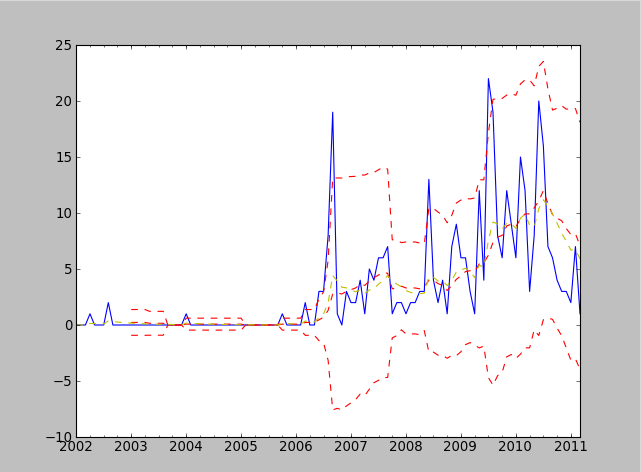
\includegraphics[width=.58\textwidth]{Bollinger.png} 
  \caption{Bollinger bönd merkt með rauðum strikalínum} 
\end{figure}
%\end{wrapfigure}


Bollinger bönd nýtast vel til að greininga hvar í
tímalínu óeðlileg hækkun eða lækkun á sér stað.




\subsection{Fourier transformations} 

Fourier umbreytingar eru stærðfræðilegar aðgerðir sem brjóta merki niður í tíðnir þess. 
Mögulegt er að umbreyta tímalínu í tíðnirit og ef ákveðin tíðni er mjög áberandi 
þá er endurtekning í tímalínunni. 

Sem dæmi um slíkt er tímalínan á mynd~\ref{fig:rafmagnsnotkun} sem sýnir
rafmagnsframleiðslu á mánuði í Evrópusambandinu.


\begin{figure}[H]
  \centering 
    \subfloat[Tímalína]{\label{fig:rafmagnsnotkun}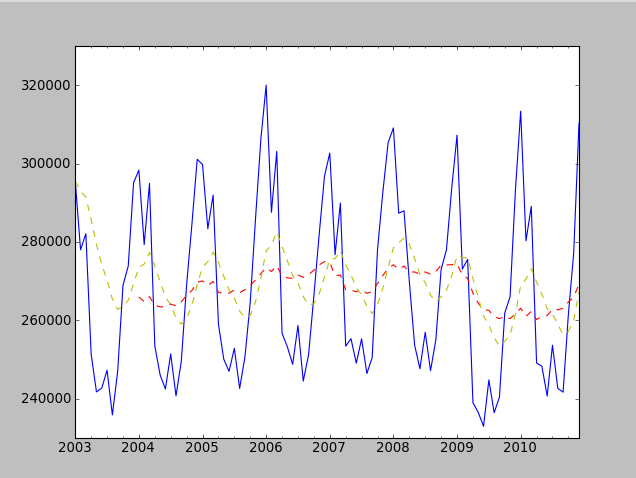
\includegraphics[width=0.42\textwidth]{Rafmagnsnotkun}}                    
     \subfloat[Tíðnirit]{\label{fig:fouriergraph}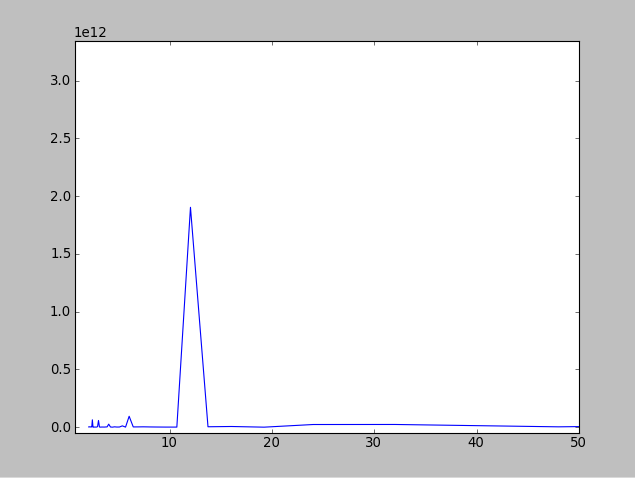
\includegraphics[width=0.42\textwidth]{Fourier}} 
      \caption{Fourier Transformations}
  \label{fig:fourier}
\end{figure}

Hér má sjá að tímalínan hefur ákveðnar endurtekningar, nánar tiltekið þá er mikil notkun á veturna en lítil á sumrin.
Þessa föstu sveiflu í tímalínunni greinir Fourier og skilar grafi eins og mynd~\ref{fig:fouriergraph} sýnir. 
Hægt er að greina að endurtekningu sem á sér stað með 12 staka millibili.

\subsection{Niðurstöður rannsókna}
Eftir að hafa rannsakað mismunandi aðferðir varð okkur ljóst að Bollinger bönd hentuðu
mjög vel fyrir flest af því sem við ætluðumst til að kerfið gerði.
Því var sett aukin áhersla á að þróa mismunandi útfærslur Bollinger banda og
dregið úr þróun annarra aðferða. 
\newpage
\section{Útfærsla}
\label{sec:imp_our}
Til að greina gögn með Bollinger böndum þarf að ákveða rammastærð.
Rammastærðin segir til um hversu langt aftur í tímann skuli litið þegar böndin eru reiknuð.
Ekki virðist vera til nein almenn leið til að áætla rammastærð útfrá gögnum tímalínunnar, það er að segja án 
nokkurra annarra fylgigagna.
Hin hefðbundna leið við ákvörðun rammastærðar er greining á atferli tímalínunnar, sú greining krefst mannlegs innsæis og því 
þurftum við að leita annarra úrræða því vandamáli.

\subsection{Reiknirit}
\label{sec:imp_algorithm}
Reiknirit Rýnis byggir grunn sinn á Bollinger böndum eins og áður hefur komið fram.
Þar sem erfitt eða ómögulegt reynist að áætla rammastærðir sjálfvirkt þá notast Rýnir við nokkrar mismunandi
rammastærðir og ítrar í gegnum þær. Hver ítrun gefur öllum punktum í tímalínu ákveðið meðaltalsvægi. Til að reikna
vægi punkts notum við okkar eigin útgáfu af formúlu sem kallast 
$\%b$\footnote[1]{Útskýringu á upprunalegu $\%b$ formúlunni og af hverju hún gagnast okkur ekki í óbreyttri mynd er að finna í tækniskýrslu á meðfylgjandi geisladisk}. 
\\ \hfil
\\ \hfil
Okkar útgáfa af $\%b$ virkar á eftirfarandi hátt:
\begin{itemize}
  \item Punktar innan bandanna fá einkunn á bilinu 0-1
  \item Punktar utan bandanna fá einkunn sem samsvarar hlutfallslegri fjarlægð frá meðaltali rammans, sem er ávallt stærri en 1.
\end{itemize}


Hér fyrir neðan er síðan formúlan okkar:


\begin{center}
  $\%b=abs(\frac{item - avg}{upperlim - avg})$
\end{center}

Einkunnirnar eru lagðar saman úr öllum rammastærðum og meðaltal þeirra fundið.
Þegar litlar breytingar eiga sér stað yfir tímabil sem er lengra en rammastærðin eiga
Bollinger böndin til með að þrengjast mikið. Það gerði það að verkum að smávægilegar breytingar eftir
rólegt tímabil fengu óeðlilega hátt gildi. 
Vægi punktsins er því minnkað ef bandbreiddin reynist óeðlilega þröng miðað við meðalbandbreidd
tímalínunnar.
Algengt er að ef tímalína rís eða fellur hratt, þá eru margir punktar í röð
taldir áhugaverðir, sem er mjög eðlilegt.
Kerfið býður þó upp á þann möguleika að skila einungis áhugaverðasta punktinum
úr röð samliggjandi punkta.

\subsection{Annmarkar}

Rannsóknir okkar leiddu í ljós að þessi aðferð hentar ekki á allar tímalínur.
Þar má til dæmis nefna línur sem innihalda mikinn fjölda punkta.
Líta má á að þær tímalínur hafi \ilqq hærri\irqq \hspace{1pt} upplausn en þær sem innihalda fáa punkta. 
Í þeim flaggar kerfið okkar punkta sem vissulega eru mjög
áhugaverðir séu þeir skoðaðir í því samhengi sem kerfið okkar sér þá þ.e. innan
rammans. Sé ramminn lítill er hægt að bera það saman við að kerfið sé að skoða
tímalínuna úr lítilli fjarlægð. Aftur á móti sé sama tímalína skoðuð úr meiri
fjarlægð getur línan virst svo gott sem flöt og því í heildina óáhugaverð.

Önnur tegund sem kerfið grípur ekki væri tímalína sem hækkar töluvert upp í ákveðinn
hápunkt og taki svo að lækka aftur niður í fyrri gildi. Gerist þetta með nógu
litlum breytingum á milli punkta er ólíklegt að kerfið okkar sjái nokkuð
athugavert við þetta þó að mögulega hafi eitthvað merkilegt átt sér stað. 
Í þessum tilvikum þyrfti að skoða tímalínurnar út frá því hvort
það eigi sér stað breyting í hinu almenna ferli tímalínunnar. Bollinger böndin
eru ekki mjög gagnleg til þess, þar sem útkoman byggir að miklu leiti á hvaða
rammastærð er notuð. 

Fjallað verður um aðferðir sem gagnast við að skoða þessa eiginleika í kafla~\ref{sec:future_linear}


\newpage
\section{Rýnir}
\subsection{Flæðirit}
\label{sec:flow_chart}

\begin{figure}[H]
  \centering
  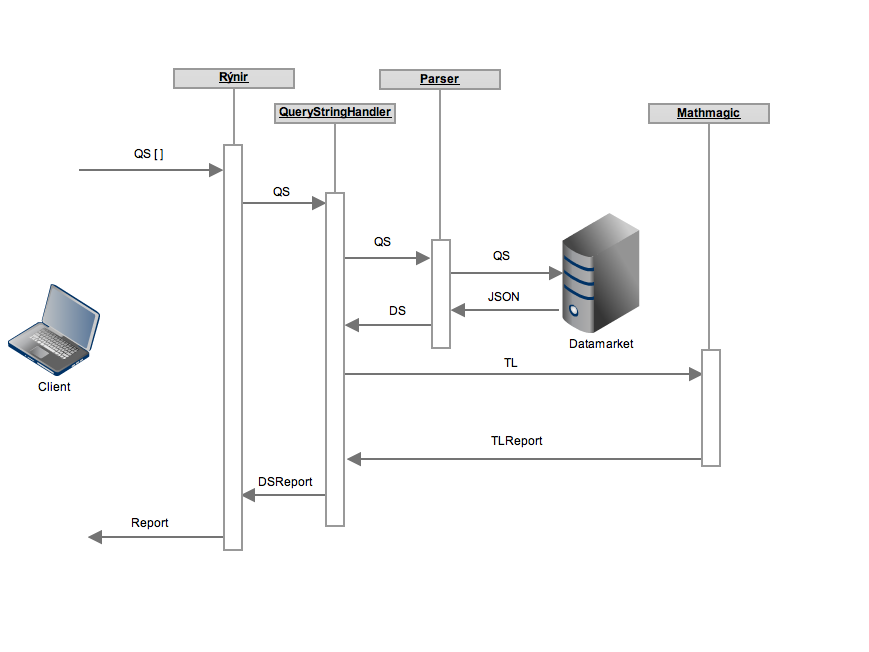
\includegraphics[width=.85\textwidth]{rynir_sequence-2.png} 
  \caption{Flæðirit} 
  \label{fig:sequence}
\end{figure}
Á mynd~\ref{fig:sequence} má sjá flæðirit fyrir Rýnir.
Kerfið tekur við lista af fyrirspurnarstrengjum
\footnote[1]{Hver fyrirspurnarstrengur stendur fyrir eitt gagnasett, hægt er að nálgast nánari lýsingar um fyrirspurnarstrengi DataMarket á http://datamarket.com/api/v1/}
\footnote[2]{Táknað á mynd~\ref{fig:sequence} sem QS[]} 
og skilar til baka skýrslu um niðurstöður. Hver fyrirspurnarstrengur er sendur til QueryStringHandler til greiningar.
Þar sér Parser klasinn um að sækja gagnasettið\footnote[3]{Táknað á mynd~\ref{fig:sequence} sem JSON} frá þjóni DataMarket
og skila því í formi sem hentar frekari vinnslu\footnote[4]{Táknað á mynd~\ref{fig:sequence} sem DS}.
MathMagic greinir hverja tímalínu í gagnasettinu og skilar lista af flöggum\footnote[4]{Táknað á mynd~\ref{fig:sequence} sem TLReport} 
sem QueryStringHandler tekur saman og skilar \footnote[4]{Táknað á mynd~\ref{fig:sequence} sem DSReport}.

Að neðan má svo sjá klasarit fyrir Rýnir.

\begin{figure}[H]
  \centering
  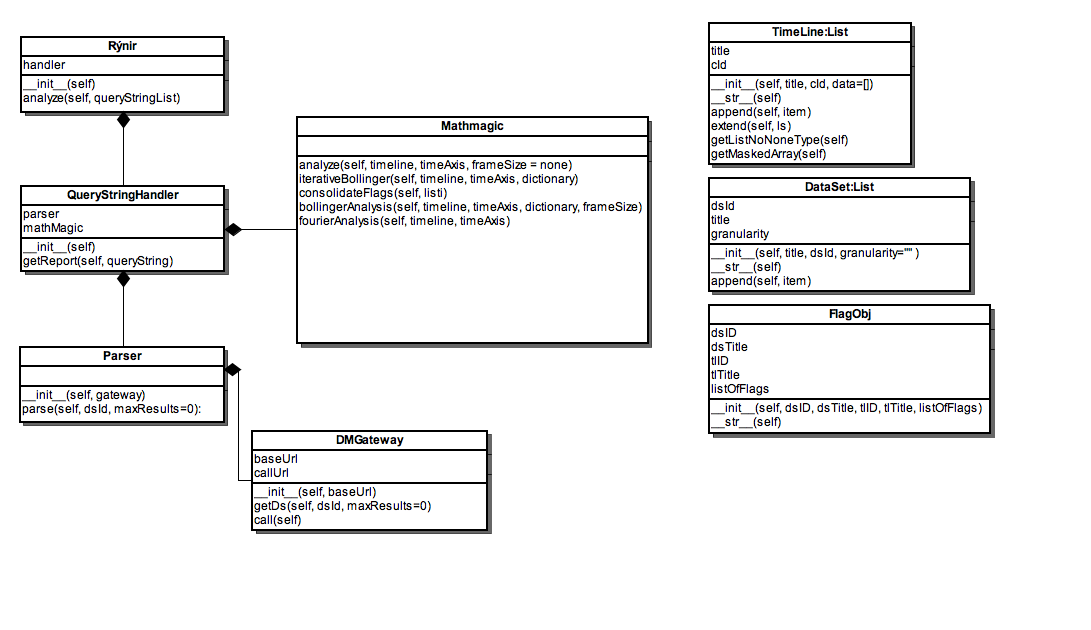
\includegraphics[width=.95\textwidth]{rynir_class_diagram.png} 
  \caption{Klasarit} 
\end{figure}
\newpage
\section{Horft til framtíðar}
\label{sec:future}

\subsection{Linear Regression}
\label{sec:future_linear}
Linear regression reynir að draga eins fáar beinar línur og hægt er í gegnum ferli tímalínunnar.
Sé hægt að gera það með einni línu má líta svo á að engin stórvægileg breyting 
eigi sér stað í almenna ferlinu og því í heild sinni sé tímalínan óáhugaverð. 
Sé ekki hægt að gera það með einni línu hefur átt sér stað nægileg breyting og má þá líta á skurðpunkt línanna sem
hugsanlega áhugaverðan punkt í tímalínunni.

\subsection{Fourier Transformation}
\label{sec:future_fourier}
Eins og fjallað var um í kafla~\ref{sec:research} nýtist Fourier
Transformation við að finna endurtekningar í tímalínum með því að brjóta þær
niður í tíðnir sínar.  
Einnig væri ekki einungis hægt að finna hvort það eigi sér stað endurtekning í
tímalínunni, heldur hvar. Þannig væri mögulegt að skoða endurtekningarnar nánar,
t.d. út frá því hvort ein endurtekningin sé óeðlilega há eða lág, eða hvort hana
hreinlega vanti eitt árið.

\newpage
\section{Framvinda}
Eins og fram kom í kafla~\ref{sec:sprettir} skiptist verkefnið upp í níu spretti. 
Hér bera að líta stutt yfirlit um hvað var gert í hverjum þeirra. Nánari upplýsingnar 
er að finna í framvinduskýrslu á meðfylgjandi geisladisk.

Myndir~\ref{fig:sp1} til~\ref{fig:sp8} 
sýna burndown rit fyrir viðkomandi spretti. Á þeim tákna grænar súlur hversu marga tíma var 
unnið viðkomandi dag og rauðar þær breytingar sem urðu á áætlun, hvort tímum var bætt við eða 
þeir dregnir frá. Blá línan sýnir framgang verksins og ljósa línan er höfð til viðmiðurnar 
við áætlun.

\subsection{Sprettur 0}
Sprettur 0 var til undirbúnings. Ekki voru sögur eins og í
hefbundnum spretti heldur var skipulögð verkáætlun, gerð áhættugreining og unnið að ýmsum öðrum
undirbúningi.
\newpage
\subsection{Sprettur 1}
Í fyrsta spretti fórum við í að kynna okkur tæknileg atriði sem við ætluðum að
nota.
Flest þeirra þekktum við, en höfðum ekki unnið með í Python áður. Þetta voru hlutir
eins og prófanadrifin þróun, REST-ful þjónustur og hvernig 
unnið er með JSON skrár. Einnig settum við upp grunn að kerfinu sem gat sótt
gögn frá DataMarket. Náðum ekki alveg að klára það sem við lögðum 
upp með og urðum að færa hluta úr sögum yfir í næsta sprett.
\hfil \\
\hfil \\
\hfil \\
\begin{figure}[H]
  \centering
  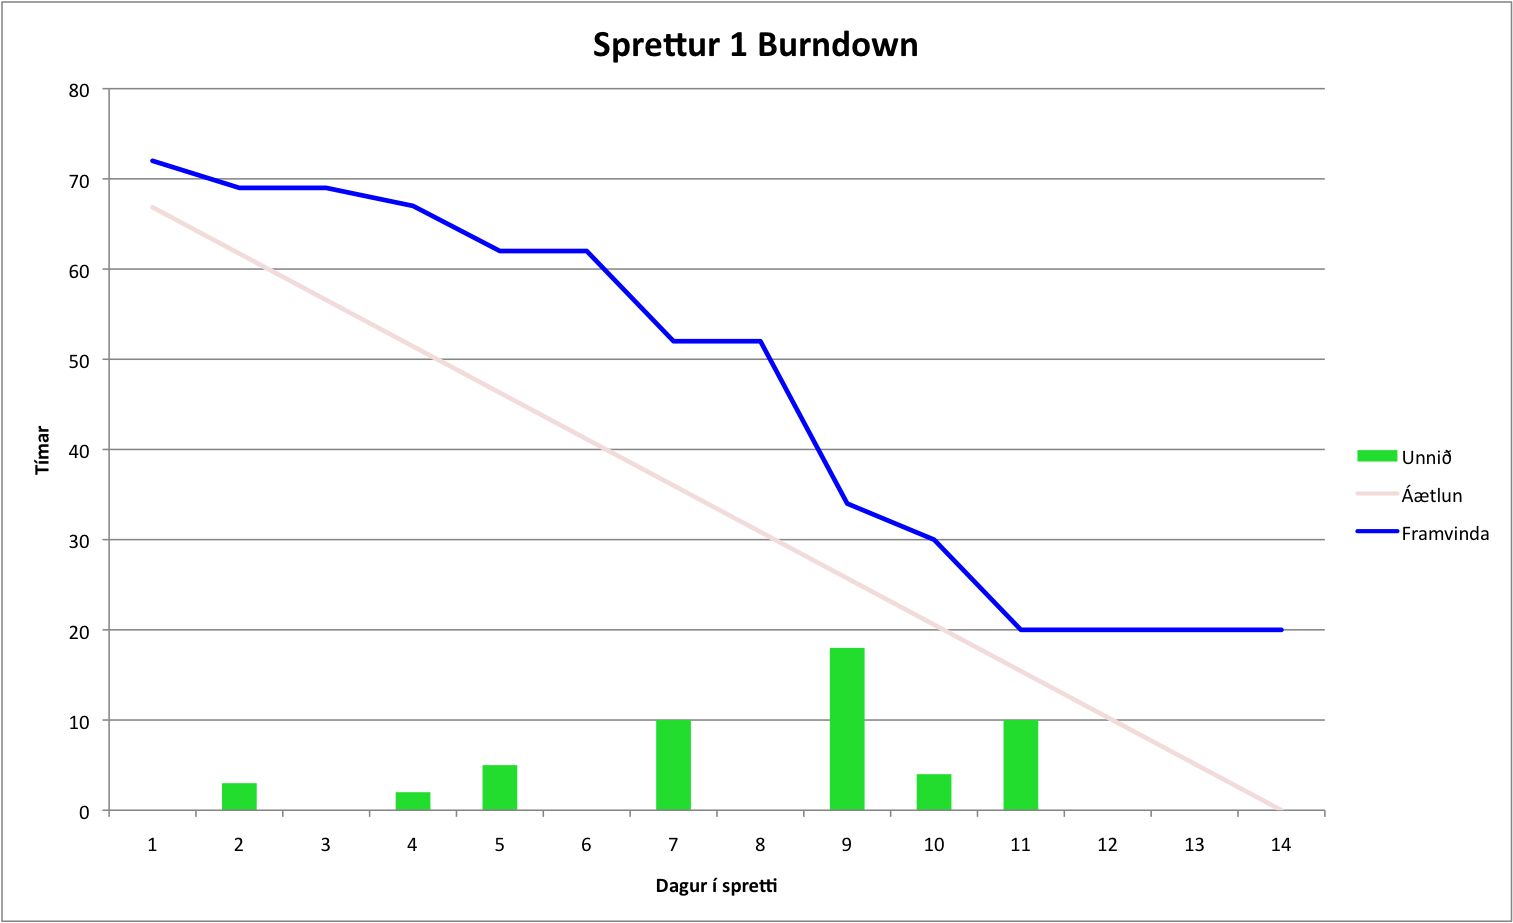
\includegraphics[width=0.72\textwidth]{Sprettur1_Burndown.png}
  \caption{}
  \label{fig:sp1}
\end{figure}
\newpage
\subsection{Sprettur 2}
Í öðrum fundum við áhugaverð gögn hjá DataMarket og settum upp staðbunda
gátt (e. service stub) svo að það myndi ekki hindra okkur í þróun ef 
aðgangur að gagnagrunni DataMarket væri ekki til staðar. Þetta var hluti af
okkar áhættugreiningu\footnote[1]{Sjá nánar í skjali um áhættugreiningu á meðfylgjandi geisladisk}. 
Þá útfærðum við fyrstu reikniaðferðirnar sem reiknuðu meðaltal, miðgildi og staðalfrávik
og létum kerfið sækja gögn og skila niðurstöðum.
Einnig áttum við fundi með sérfræðingum á sviði stærðfræði og tölfræði, til að ýta
úr vör hugmyndavinnu fyrir seinni fasa.
\hfil \\
\hfil \\
\hfil \\
\begin{figure}[H]
 \centering
 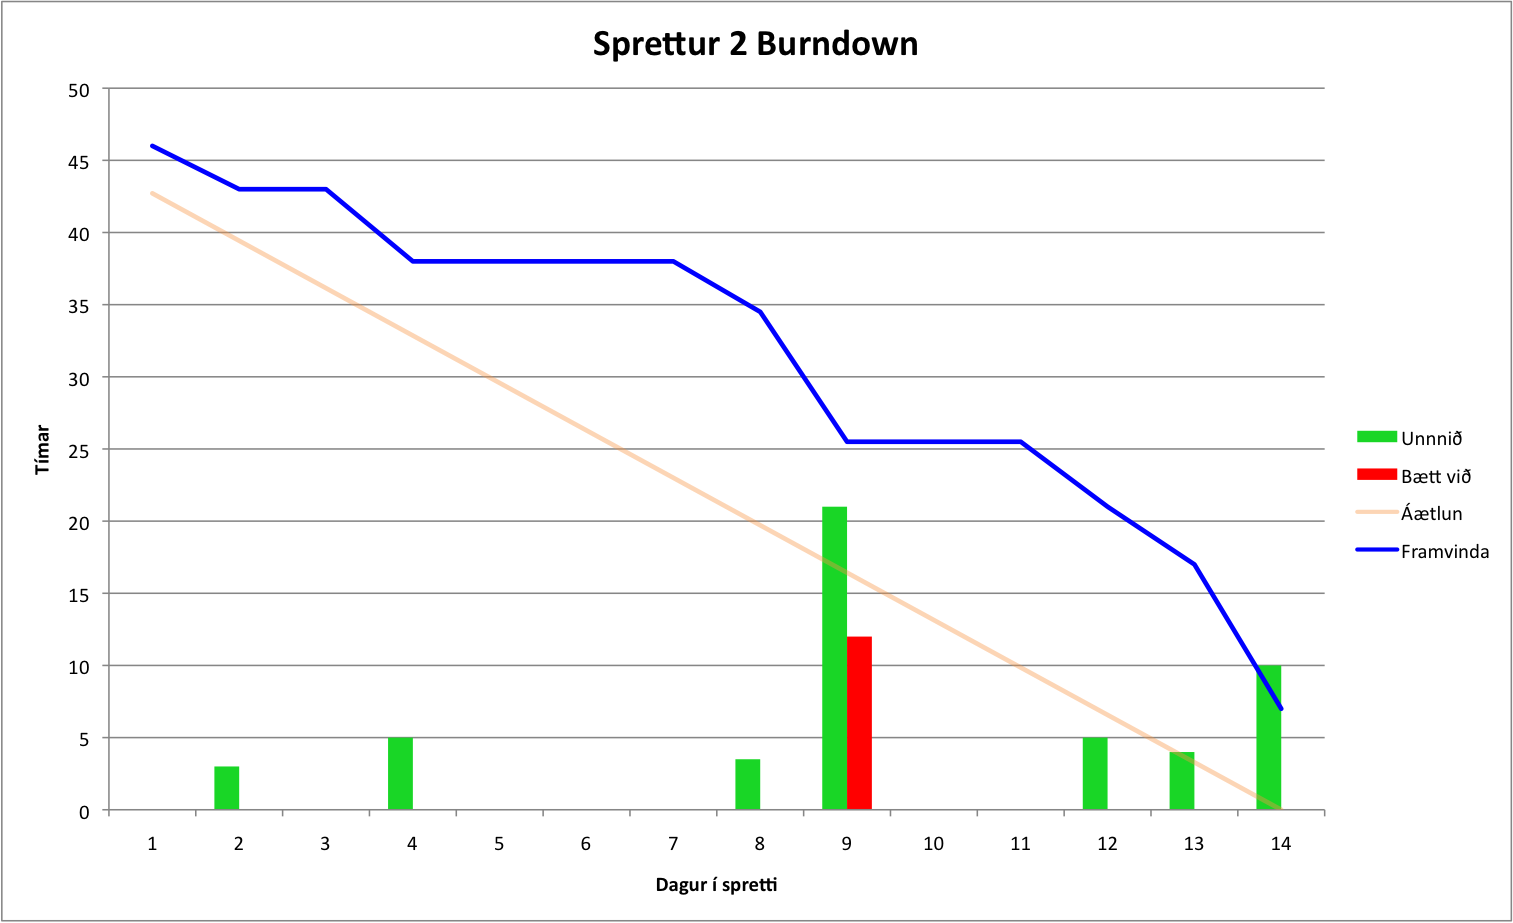
\includegraphics[width=0.72\textwidth]{Sprettur2_Burndown.png}
 \caption{}
\end{figure}
\label{fig:sp2}
\newpage
\subsection{Sprettur 3}
Þegar hér var komið við sögu vorum við farnir að finna ákveðinn takt í
áætlanagerð og sáum betur hvað við gátum gert ráð fyrir að klára mikið 
í einum sprett. Við settum upp aðgerðarsöfn (e. libraries) sem voru til þess fallin að
aðstoða okkur við útreikninga. Það tók þó umtalsvert lengri tíma en við gerðum
ráð fyrir. Þá bættum við staðbundnu gáttina og kynntum okkur aðgerðarsöfnin.
Hugmyndavinnu að frekari reikniaðgerðum var haldið áfram.
\hfil \\
\hfil \\
\hfil \\
\begin{figure}[H]
 \centering
 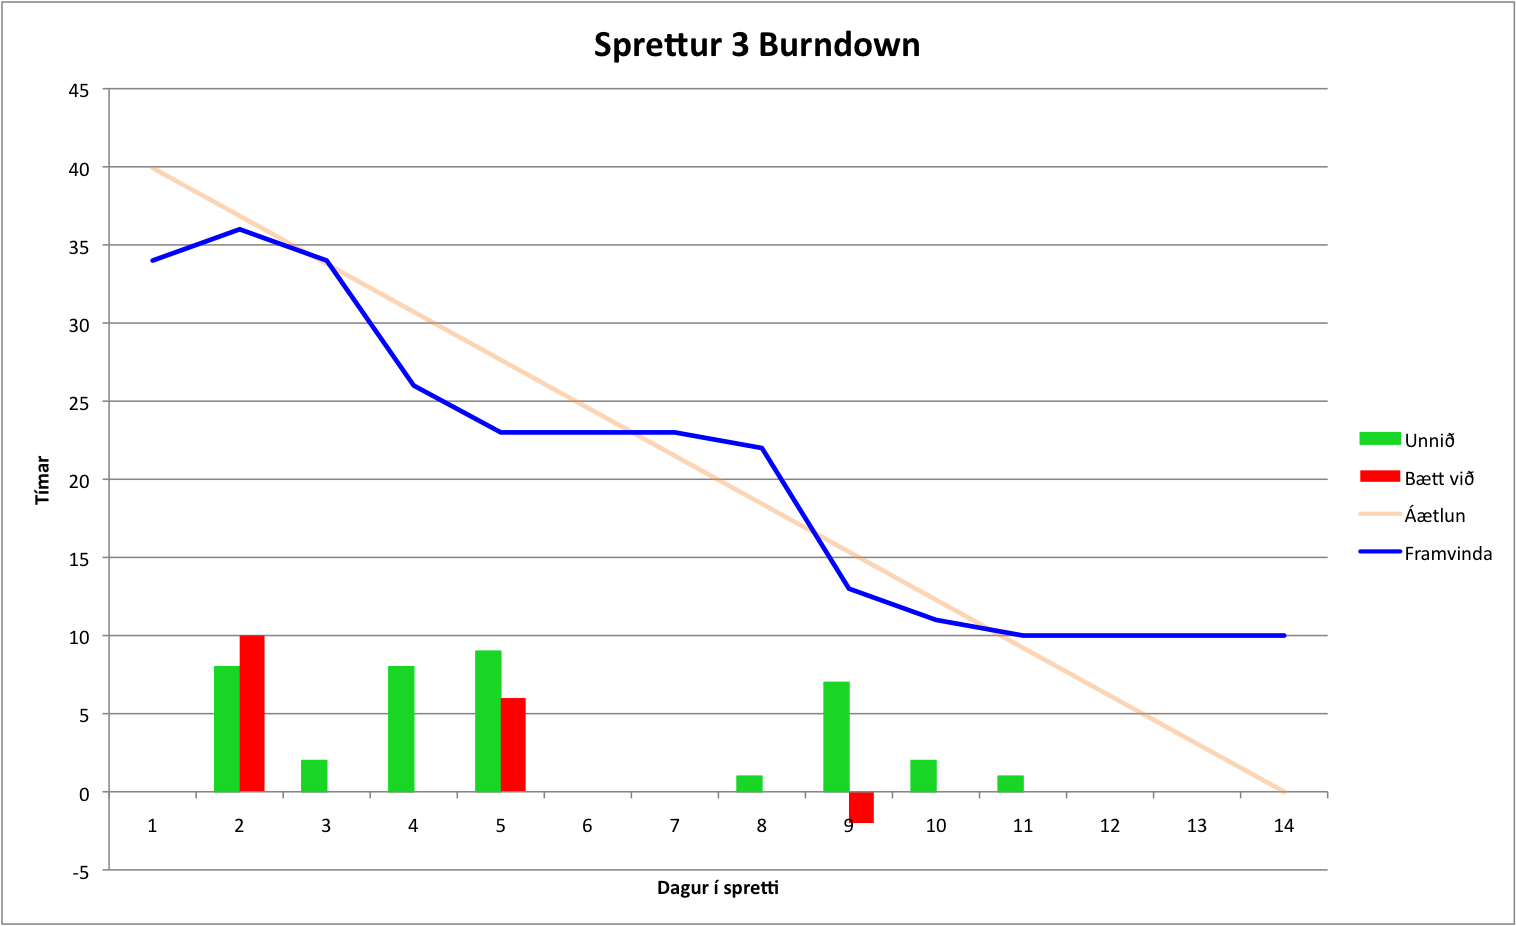
\includegraphics[width=0.72\textwidth]{Sprettur3_Burndown.png}
 \caption{}
\end{figure}
\label{fig:sp3}
\newpage
\subsection{Sprettur 4}
Spretturinn fór í að setja upp framenda á kerfið og ákvarða úttak kerfisins. 
Þegar við vorum svo farnir að nota aðgerðarsöfnin 
kom á daginn að einföldu aðferðirnar okkar voru mun betri en vonir stóðu til.
Einnig komumst við að því að það hafa aðrir beitt þessum aðferðum 
og kallast þær Bollinger bönd, sjá nánar kafla~\ref{sec:research_bollinger_bands}. 

Við gátum nú sýnt þeim hjá DataMarket niðurstöður úr kerfinu okkar og við það
urðu til fleiri hugmyndir um hvernig hægt væri að nýta það (sjá kafla~\ref{sec:description}).

Fáir sögupunktar voru settir í sprettinn og hann kláraður snemma þar sem lokapróf voru framundan.
\hfil \\
\hfil \\
\hfil \\
\begin{figure}[H]
 \centering
 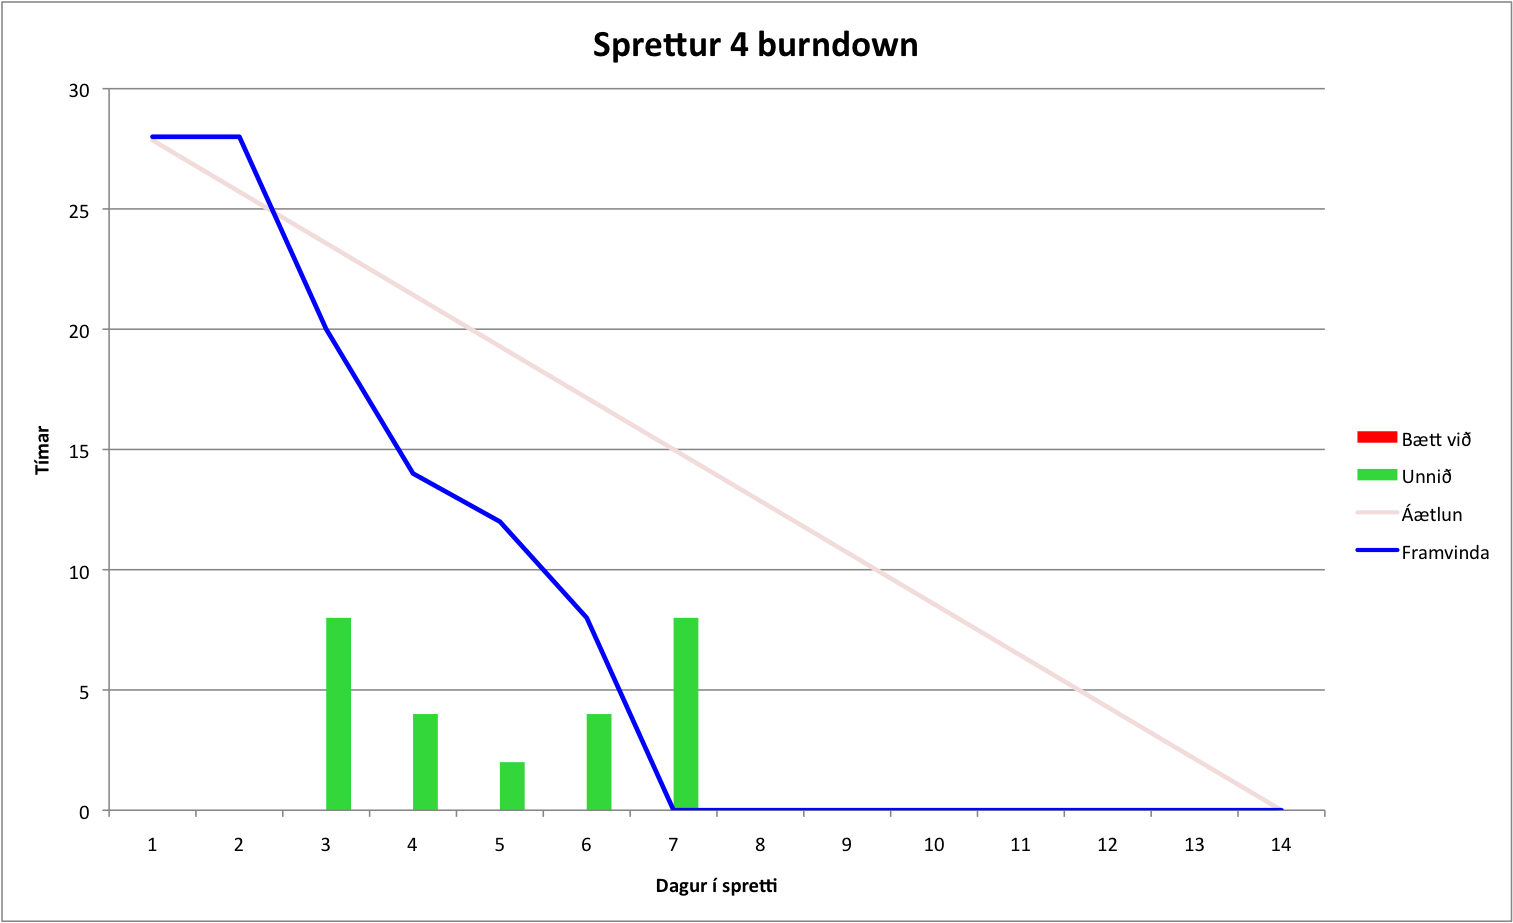
\includegraphics[width=0.72\textwidth]{Sprettur4_Burndown.png}
 \caption{}
\label{fig:sp4}
\end{figure}
\newpage
\subsection{Sprettur 5}
Síðasti sprettur í fyrri fasa. Funduðum með DataMarket og ákváðum endanlegt form á
flöggum sem er skilað. Gengum frá lausum endum, kóði yfirfarinn 
(e. refactor) og fyrsta útgáfa varð til. Hugmyndavinna fyrir annan fasa komin vel á veg.
\hfil \\
\hfil \\
\hfil \\
\begin{figure}[H]
 \centering
 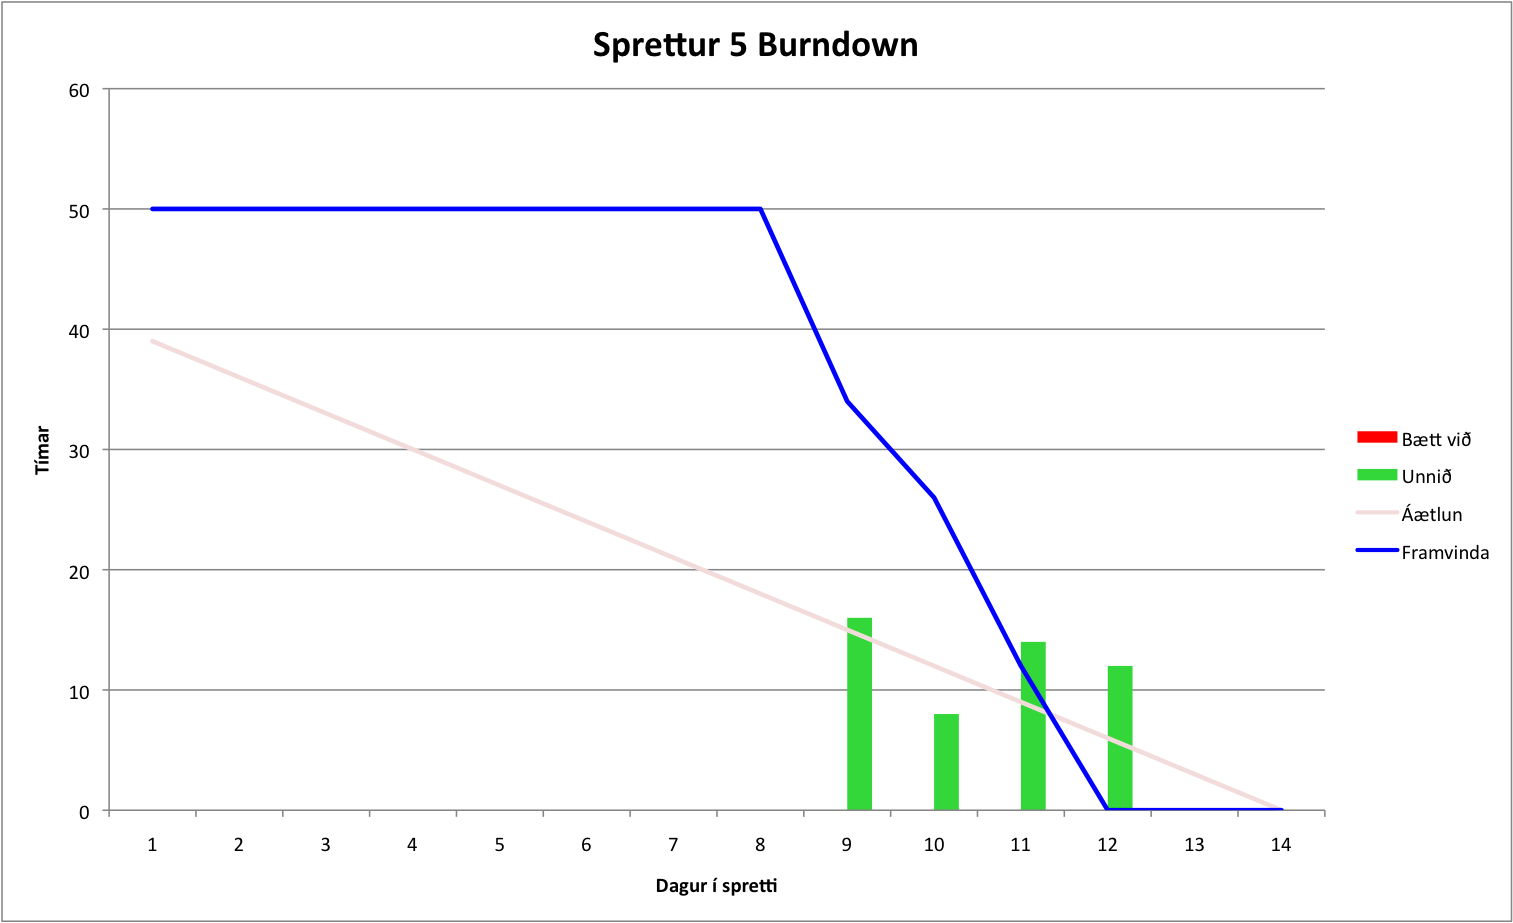
\includegraphics[width=0.72\textwidth]{Sprettur5_Burndown.png}
 \caption{}
\label{fig:sp5}
\end{figure}
\newpage
\subsection{Sprettur 6}
Við höfðum sankað að okkur mikið af upplýsingum og höfðum ákveðnar hugmyndir um
hvað okkur langaði að gera. Það krafðist þess hinsvegar að við 
þurftum að framkvæma prófanir til að sjá hvað myndi henta okkar kerfi best. 
Af þeim sökum voru fáar sögur fullmótaðar, en þeim bætt við þegar líða tók á sprettinn.
Vinna við lokaskýrslu hófst. Í lok sprettsins vorum við komnir með verulega bættar reikniaðgerðir frá því sem var.
\hfil \\
\hfil \\
\hfil \\
\begin{figure}[H]
 \centering
 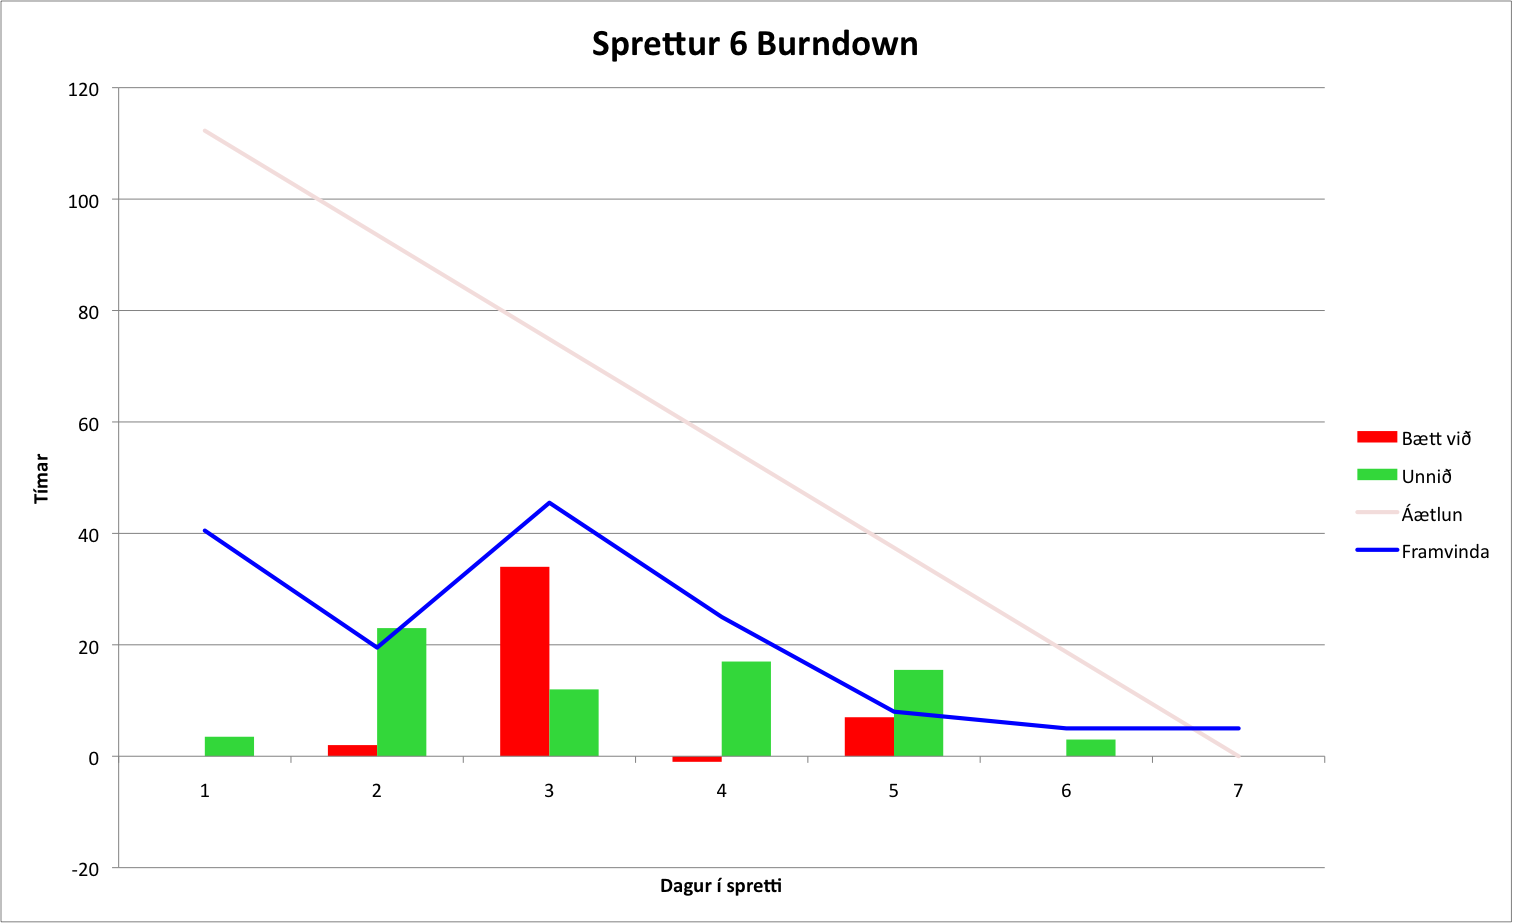
\includegraphics[width=0.72\textwidth]{Sprettur6_Burndown.png}
 \caption{}
\label{fig:sp6}
\end{figure}
\newpage
\subsection{Sprettur 7}
Byrjað á lokafrágangi. Allar keyrslustillingar lesnar úr skrá og villumeðhöndlun
yfirfarin. Sett upp villu og athugasemdakerfi (e. logging system). Framkvæmdum álagsprófanir og 
yfirfórum niðurstöður úr þeim. Fínstillingar á reikniritum og villur lagfærðar. 
\hfil \\
\hfil \\
\hfil \\
\begin{figure}[H]
 \centering
 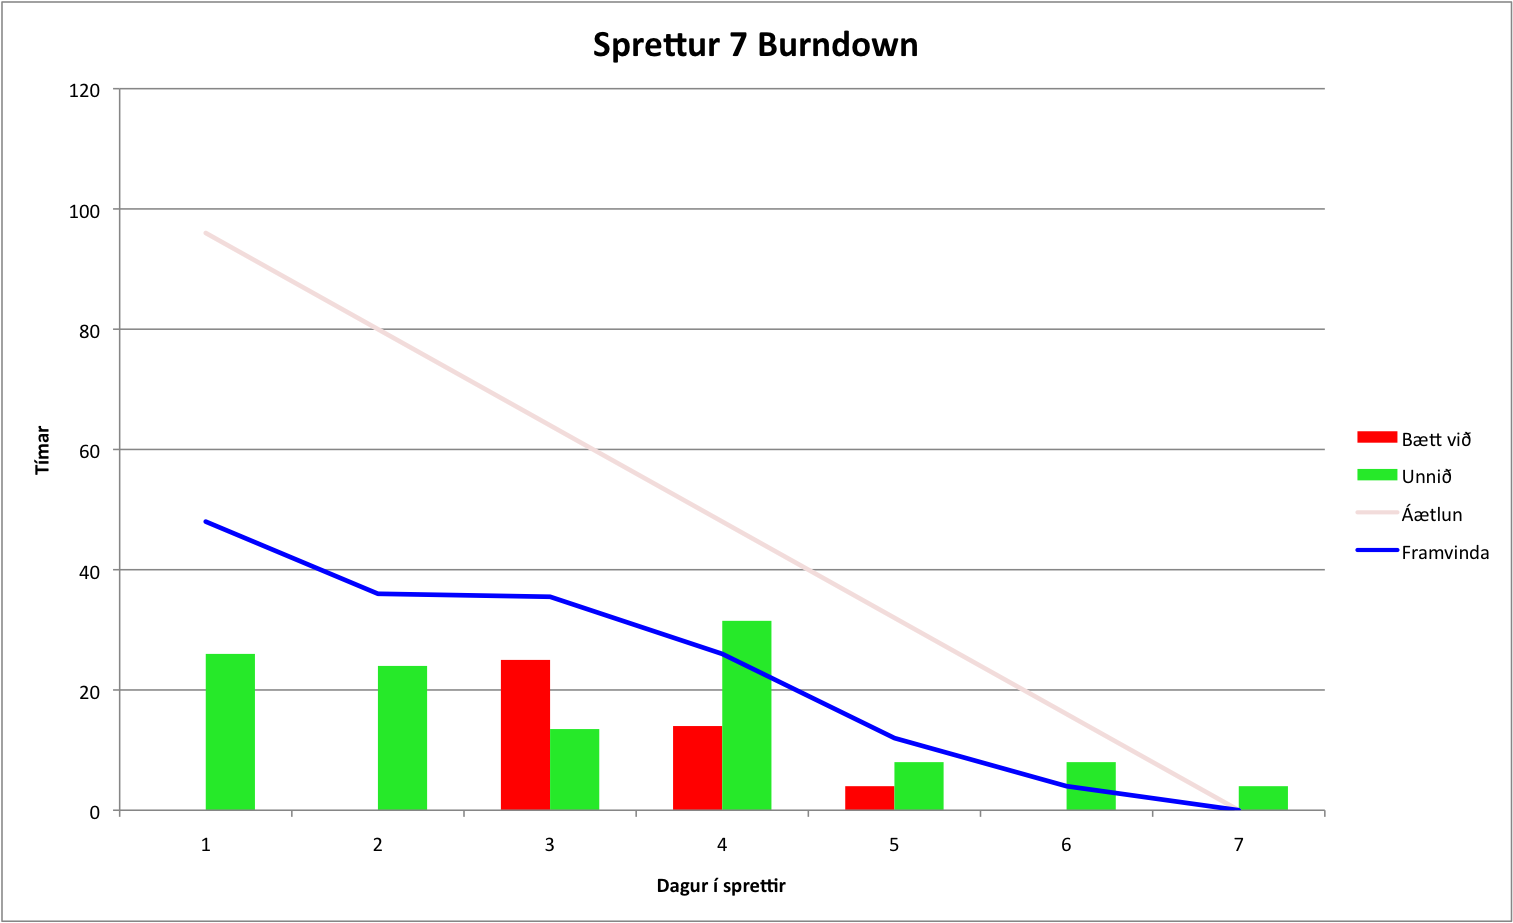
\includegraphics[width=0.72\textwidth]{Sprettur7_Burndown.png}
 \caption{}
\label{fig:sp7}
\end{figure}
\newpage
\subsection{Sprettur 8}
Skýrslugerð í forgangi. Lokafrágangur á kóða. Læddum inn einni
bætingu á reikniaðferðum og prófuðum uppá nýtt.
\hfil \\
\hfil \\
\hfil \\
\begin{figure}[H]
 \centering
 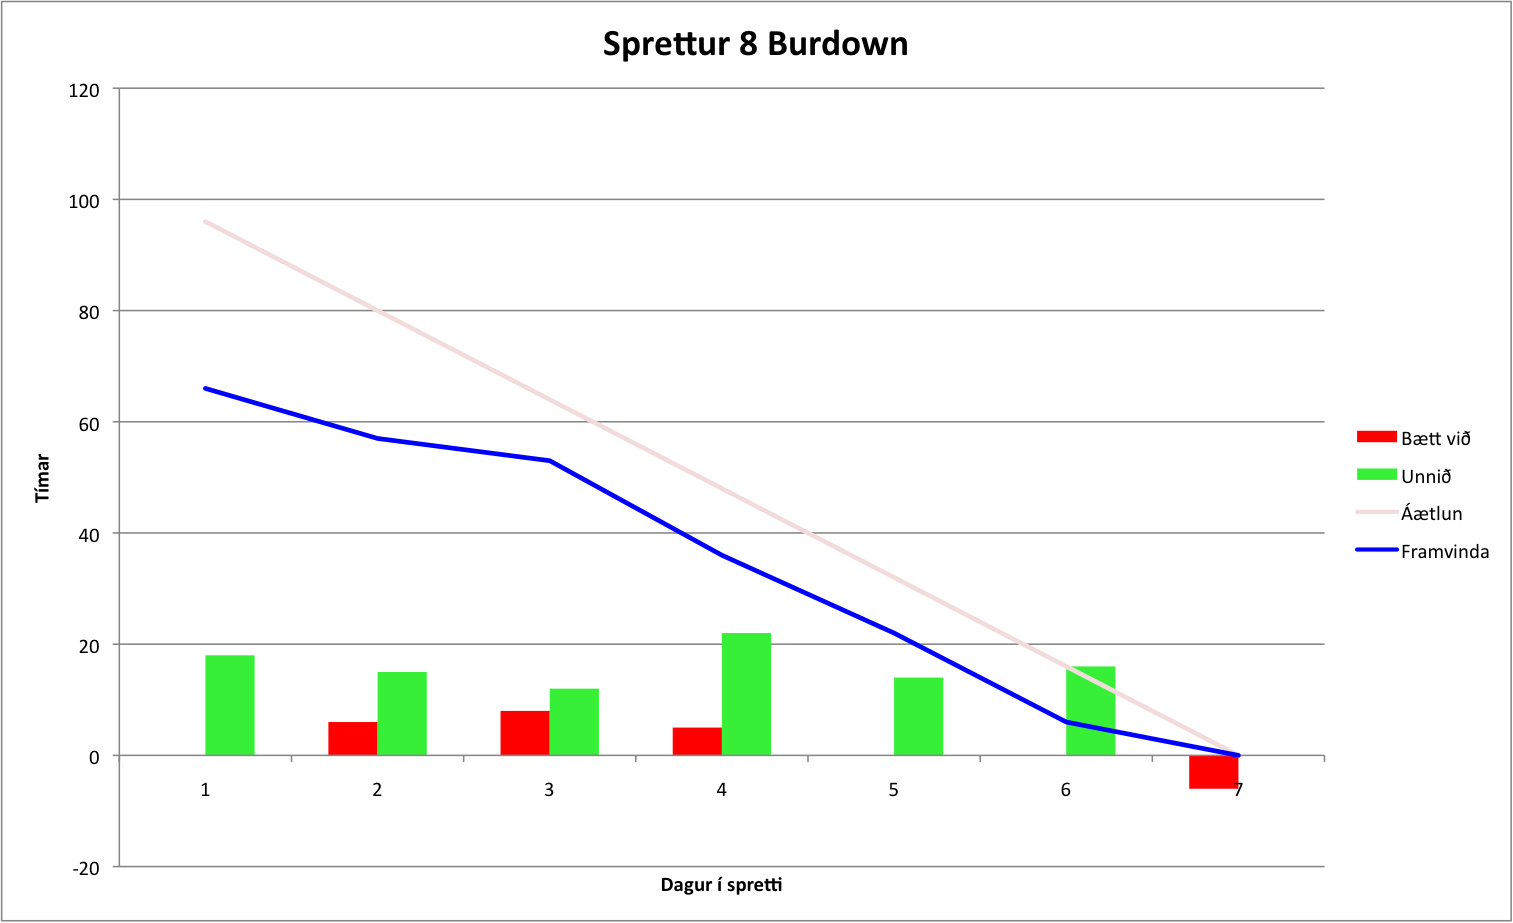
\includegraphics[width=0.72\textwidth]{Sprettur8_Burndown.png}
 \caption{}
\label{fig:sp8}
\end{figure}

\hfil \\
\hfil \\
\hfil \\
\hfil \\

\section{Lokaorð}
Verkefnið var mjög opið enda upphaflegt markmið að finna áhugaverð gögn. 
Út frá því fóru af stað miklar vangaveltur um hvað teldist til áhugaverðra gagna. 
Okkur þótti gaman að sjá kerfið þróast frá hugmynd að fullkláraðri afurð sem DataMarket getur nýtt sér.
Við sáum það svart á hvítu hversu mikilvægt er að beita skipulögðum aðferðum við að komast að settu markmiði og má þá helst nefna hvernig
við nýttum okkur Scrum og samstæðustjórnun. Þegar litið er til baka erum við ánægðir með hversu vel okkur gekk að leysa 
vandamál sem komu upp en hópurinn sameinaðist í að greina og leysa vandann strax og hann kom upp.
Hópurinn er sammála um að verkefnið hafi gengið vel og að niðurstöður Rýnis séu vissulega ábendingar á áhugaverð gögn.
Vinna hópsins leiddi einnig af sér tillögur að frekari þróun Rýnis sem ómögulegt reyndist að útfæra sökum tímaramma verkefnisins.
Því ætti verkefnið í heild sinni að gagnast DataMarket til frekari greiningar á tölfræðilegum gögnum.

Þetta gaf okkur góða tilfinningu fyrir því að námið muni gagnast okkur vel í atvinnulífinu. 



\end{document}